 \documentclass[12pt]{article}

\usepackage[margin=1in]{geometry}
\usepackage{fancyhdr}
\usepackage{setspace}
\pagestyle{fancy}
\usepackage{amsmath, amsthm, amssymb, amsfonts, mathtools, xfrac,mathrsfs}
\usepackage[utf8]{inputenc}
\usepackage[english]{babel}
\usepackage{graphicx,dsfont}
\usepackage{braket, bm}

\everymath{\displaystyle}
\headheight=20pt


\newcommand{\N}{\mathbb{N}}
\newcommand{\Z}{\mathbb{Z}}
\newcommand{\Q}{\mathbb{Q}}
\newcommand{\R}{\mathbb{R}}
\newcommand{\E}{\mathrm{E}}
\newcommand{\Var} {\mathrm{Var}}
\newcommand{\Cov}{\mathrm{Cov}}
\newcommand{\F}{\mathbb{F}}

\DeclareMathOperator{\Tr}{Tr}

\def\mean#1{\left< #1 \right>}
 
\newcommand*\rfrac[2]{{}^{#1}\!/_{#2}}
 
\newenvironment{theorem}[2][Theorem]{\begin{trivlist}
\item[\hskip \labelsep {\bfseries #1}\hskip \labelsep {\bfseries #2}]}{\end{trivlist}}

\newenvironment{problem}[2][Problem]{\begin{trivlist}
\item[\hskip \labelsep {\bfseries #1}\hskip \labelsep {\bfseries #2}]}{\end{trivlist}}

\title{Homework}
\lhead{Math OSM Lab}
\chead{Homework 6 - 8/31/17}
\rhead{Dan Ehrlich}
 
\begin{document}

\begin{problem}{8.1.} We graph the feasible set below. To find the optimizer, plot the objective function over the feasible set and find the maximum point. The optimizer is at $(14/5, 16/5)$ and the objective function has a value of $6/5$. 
\begin{center}
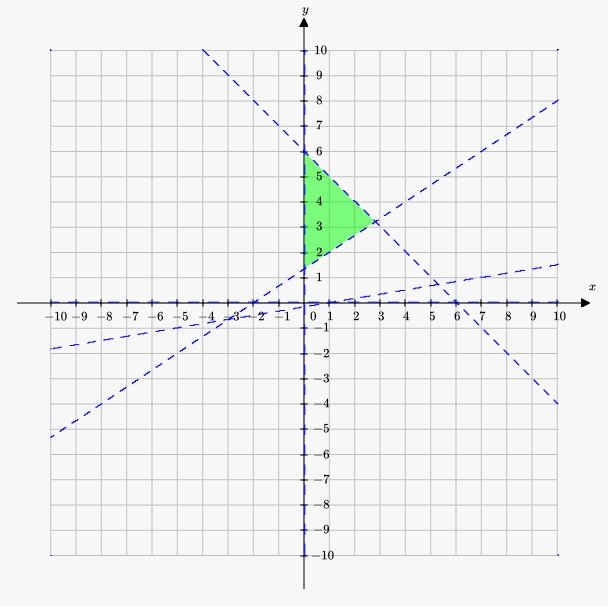
\includegraphics[width=8cm, height=8cm]{prob1.jpeg}
\end{center}
\end{problem}

\begin{problem}{8.2.}\hfill
\begin{itemize}
\item[(i)]We graph the feasible set below. The optimizer is at $(6, 2)$ and the objective function has a value of $20$. 
\begin{center}
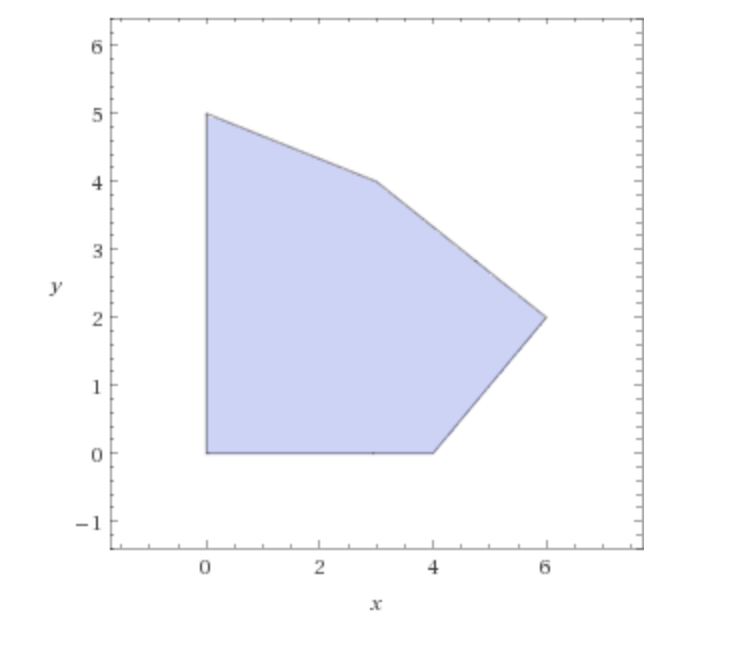
\includegraphics[width=8cm, height=8cm]{prob8i}
\end{center}
\item[(ii)]We graph the feasible set below. The optimizer is at $(15, 12)$ and the objective function has a value of $132$. 
\begin{center}
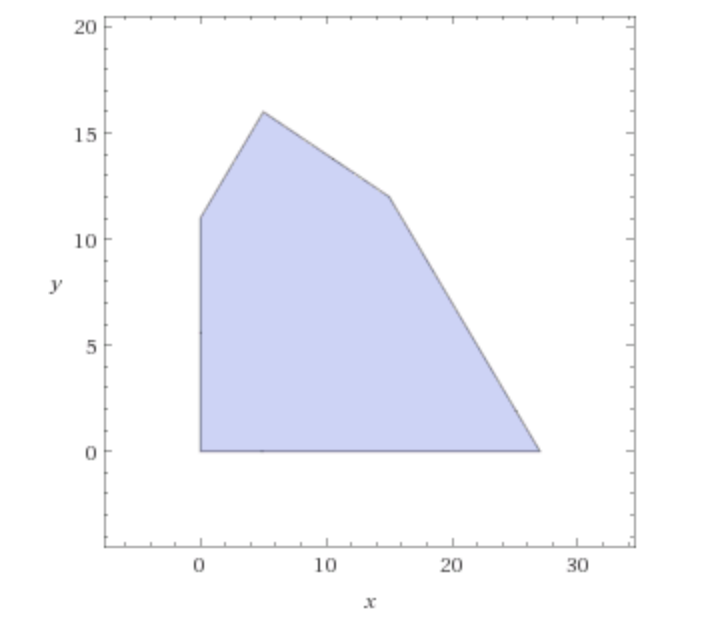
\includegraphics[width=8cm, height=8cm]{prob8ii}
\end{center}
\end{itemize}
\end{problem}

\begin{problem}{8.5.}
\end{problem}

\begin{problem}{8.7.} 
\end{problem}

\begin{problem}{8.13.} 
\end{problem}

\begin{problem}{8.17.} 
\end{problem}

\begin{problem}{8.18.} 
\end{problem}

\begin{problem}{9.3.}
\end{problem}

\begin{problem}{9.6.}
\end{problem}

\begin{problem}{9.7.}
\end{problem}

\begin{problem}{9.10.}
\end{problem}

\end{document}

